\newpage
\begin{center}
  \textbf{\large 1. АНАЛИЗ ПРЕДМЕТНОЙ ОБЛАСТИ}
\end{center}
\refstepcounter{chapter}
\addcontentsline{toc}{chapter}{1. АНАЛИЗ ПРЕДМЕТНОЙ ОБЛАСТИ}


\section{Общие сведения об области распознавания речи}

В настоящее время существуют разные подходы к разработке систем распознавания речи и улучшения их качества.
Но прежде чем перейти к описанию методов, необходимо уточнить, как происходит оценка качества работы моделей.
В чём-то расчёт метрик похож на тот же из текстовых задач.
Нам необходимо оценить похожесть сгенерированной последовательности относительно какого-то референсного текста.
Отличием является то, что если в задачах машинного перевода и написания текста порядок слов может играть роль в плане правил языка, но вместе с тем может быть допустимо, чтобы слова были в другом порядке.
Переставлять слова в аудио мы по понятным причинам не можем.

Основным методом для оценки качества работы алгоритма создания текстовой транскрипции для аудио используют расстояние Левенштейна.
Данная метрика подсчитывает своеобразный замер расстояния между отдельными элементами последовательности.
Или же другими словами цену перевода сгенерированного текста в референсный.
В общем виде на основе двух текстовых последовательностей: целевой и полученной алгоритмом машинного обучения -- идёт расчёт четырёх числовых метрик, которые затем подставляются в формулу.
Метрика принимает значения в диапазоне $[0, +\inf]$, где 0 - последовательности идентичны.
Общая формула представлена в уравнение~\ref{eq:levinstein}:

\begin{equation}
  Levenstein Distance = \frac{S + D + I}{N} = \frac{S + D + I}{S + D + C}
  \label{eq:levinstein}
\end{equation}


где $S$ обозначает количество замен, $D$ - удалений, $I$ - вставок и $C$ - правильных слов, а $N$ - всего слов в референсе. 
Если количество слов в исходной и полученной последовательностях равны, но слова разные, то они считаются как замена. 
Если слов в исходной последовательности больше, то разница считается как удаление.
Для случая, когда количество слов в изначальной последовательности больше, чем в сгенерированной, разница будет считаться как вставка.
И случаи, когда слова в обеих последовательностях совпадают, считаются как правильная транскрипция.

Как можно понять из формулы, она даёт более плохой результат в случае, когда наша модель генерирует последовательность длины сильно больше оригинальной.
Также видно, что основная разница между последовательностями замеряется с помощью $I$ и $C$, в то время как две другие величины скорее сглаживают результат.


Расстояние Левенштейна лежит в основе двух метрик, выбор между которыми сводится к выбору группы, к которой относится целевой язык:
\begin{itemize}
  \item Для китайского, японского и корейского языков используется Character Error Rate (CER), который считает расстояние между словами посимвольно.
  CER используется для групп языков, где одни и те же единицы языка в разном порядке могут давать совершенно разный результат.
  Также в этой группе один символ может отображать отдельные слова и целые явления, исторические события и легенды, поэтому тут важна точность каждой единицы языка по отдельности.
  \item Для русского, английского и немецкого используется Word Error Rate (WER), который уже считает расстояние между отдельными словами.
  Поскольку в этой группе языков буквы не играют по отдельности большой роли в формирование предложений, здесь в качестве основы для оценки качества принято использовать расстояния Левенштейна по словам.
\end{itemize}

В дальнейшем в этой работе оценка качества моделей будет проводиться на основе WER, так как мы будем оценивать качество для русского.

Датасеты требует своих подходов к предобработке и анализу в зависимости от задачи.
Например, для компьютерного зрения необходимы большие наборы размеченных изображений, а для обработки естественного языка — корпусы текстов с аннотациями.
Модели распознавания речи не берут сырое аудио для последующего распознавания речи, а сначала преобразуют его в другое представление, с которым потом и будут работать.
Зачастую в качестве такого представления выступает Mel-Spectrogram.
Рассмотрим основные этапы:
\begin{enumerate}
  \item Аудио разбивается на окна фиксированного размера с заданным шагом.
  \item Применяется функция для обработки этих окон.
  Зачастую используется функция Ханна.
  Это необходимо, чтобы после применения быстрого преобразования Фурье полученные частоты были менее зашумлёнными.
  \item Быстрое преобразования Фурье для разложения изначального сигнала на гармонические составляющие.
  Другими словами для перехода к частотам.
  \item Применение фильтра Мела.
  Так мы отбрасываем частоты, которые не могут быть распознаны человеческим ухом, а следовательно и не несут информации для задачи транскрибации аудио.
  \item Логарифмирование энергии.
\end{enumerate}

\begin{figure}[!t]
  \centering
  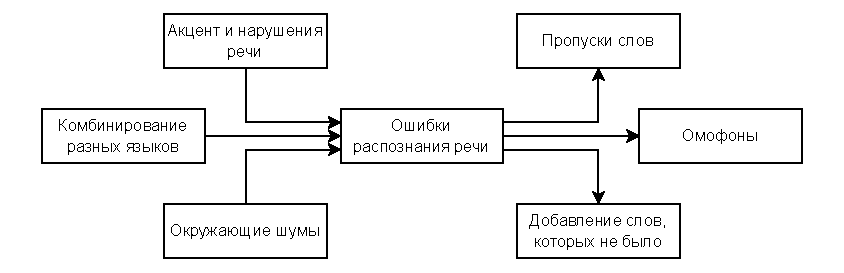
\includegraphics[width=140mm]{problems.pdf}
  \caption{Причины возникновения неточностей при распознавание речи и виды ошибок.}
  \label{fig:problems}
\end{figure}

Теперь обсудим основные причины ошибок и чем они характеризуются на Рис.~\ref{fig:problems}.

Первая и наиболее очевидная причина -- особенности произношения и нарушения речи.
Системы ASR обучаются на больших массивах данных, в котормых может преобладать «чистая» и стандартная речь, то есть записанная профессиональными дикторами.
Однако в реальности люди говорят с разными акцентами, диалектными особенностями или дефектами дикции.
Нечёткое произношение звуков, проглатывание окончаний или индивидуальные речевые привычки могут сбить алгоритм с толку.
Даже незначительные отклонения от «эталонного» произношения приводят к тому, что система либо пропускает слова, либо распознаёт их неправильно.

Вторая серьёзная проблема -- смешение языков в одной фразе.
Допустим, русский язык развивается за счёт заимствования слов и терминов из других языков.
Особенно ярко это проявляется в технической среде, где в речи встречаются как отдельные слова «фичи», «ллм» и «мл», так и целые предложения «Загрузил на сервер» или «Сделал репост», содержащие англицизмы.
Проблема, что эти слова могут отсутствовать в обучающих данных для русскоязычной модели.
ASR-системы, особенно узкоспециализированные, плохо справляются с такими переключениями, что приводит к ошибкам вроде замены слов или их полного игнорирования.

Наконец, третья распространённая причина ошибок -- фоновые шумы и акустические помехи.
Микрофоны улавливают не только голос, но и все окружающие звуки: шум транспорта или стройки, разговоры других людей, музыку или даже просто статику.
Даже продвинутые алгоритмы шумоподавления не всегда могут отделить полезный сигнал от помех, из-за чего ASR часто начинают страдать от галлюцинаций и либо добавлять лишние слова и отдельные части предложений, приняв шум за речь, либо, наоборот, пропускать фрагменты из-за искажённого звука.
Особенно критично это в условиях уличного шума или при записи с плохого микрофона.
Для решения данной проблемы даже проводится специальное соревнование под названием «CHiME Speech Separation and Recognition Challenge».
В рамках данного соревенования участники на датасете CHiME создают решения ASR, устойчивые к шумам, которые были добавлены к аудиозаписям.

Эти три фактора -- акценты и нарушения речи, смешение языков и шумовая загрязнённость аудио -- создают основные сложности для современных систем распознавания.
И хотя технологии постоянно улучшаются, полностью избавиться от ошибок пока невозможно.
Теперь рассмотрим ошибки, которые возникают из-за этих проблем.

Одной из распространенных ошибок являются пропуски слов, когда система не распознает и не включает в итоговый текст некоторые слова из исходной речи.
Это часто происходит, когда слова произносятся нечетко, слитно или слишком тихо.
Фоновые шумы также могут мешать корректному распознаванию, особенно если запись производится в неидеальных акустических условиях.
Кроме того, модель может пропускать слова, которые редко встречаются в обучающих данных или отсутствуют в ее словаре.
Предложение «Я купил молоко и хлеб» может быть преобразована в «Я купил хлеб», где слово «молоко» оказалось пропущено.

Другая типичная ошибка -- это добавление лишних слов, которых не было в оригинальной речи.
Такие ошибки часто возникают из-за артефактов аудиозаписи, например, когда посторонние шумы или эхо интерпретируются системой как речь.
В диалогах, где люди перебивают друг друга или говорят одновременно, ASR может ошибочно вставить слова, которых на самом деле не было.
Иногда языковая модель, пытаясь предсказать наиболее вероятную последовательность слов, добавляет лишние элементы.
Например, фраза «Завтра будет дождь» может превратиться в «Завтра возможно будет дождь», где слово «возможно» появилось из-за ошибки модели распознавания речи.

Особую сложность для систем распознавания речи представляют омофоны -- слова, которые звучат одинаково, но имеют разное написание и значение.
Поскольку ASR анализирует звуковую форму слов, не имея текстового контекста, система может выбрать неправильный вариант.
Пары слов «луг» и «лук» звучат идентично, но означают совершенно разные вещи.
То же самое происходит с «плот» и «плод», «код» и «кот».
Ошибки такого типа особенно критичны в специализированных областях, где точность терминов имеет большое значение.

\section{Методы машинного обучения для задачи распознавания речи}

\subsection{Функция потерь и базовые архитектуры}

Традиционно модели обучались с использованием Connectionist Temporal Classification (CTC) функции потерь.
Поскольку в аудио отдельные звуки могут занимать разные по продолжительности сегменты, встала необходимость в выравнивание этих кусочков.
Так протяжные звуки иногда необходимо объединять вместе, как-то обозначать пустоту, когда речи в аудио нет.
Проблемой CTC является то, что при декодирование отсутствует контекстная информация, так как предполагается, что токены распределны независимо.
Также качество модели сильно зависит от внешней языковой модели.

Были попытки улучшения качества за счёт архитектурных решений.
Так появились Transducer (RNN-T) и Listen, Attend, Spell (LAS).
RNN-T добавляет к аудио энкодеру ещё два компонента - предиктор и joiner-сеть.
Предиктор представляется собой каузальную сеть, основанную зачастую на рекуррентных или траснформерных сетях.
Каузальная означает, что она генерирует следующий токен, опираясь только на предыдущую информацию.
Joiner же является многослойным перцептроном.
Начальное состояние предиктора задаётся равным 0 ровно также, как оно задавалось бы при предсказание текста в рекуррентной сети.
Изначальное аудио или точнее её Мел-Спектрограмма окна кодируется в скрытое пространство с помощью аудио кодировщика.
Затем вывод кодировщика и предсказателя объединяются в полносвязной сети joiner.
Выход joiner'а представляет собой предсказание символа ASR и вместе с тем новым скрытым состоянием для предиктора.
Далее сеть повторно генерирует следующий токен и передаёт новое состояние в предиктор до тех пор, пока все окна аудио не будут переведы в символы.
Архитектуры на CTC и Transducer можно посмотреть на Рис.~\ref{fig:ctc_t}.

\begin{figure}[!t]
  \centering
  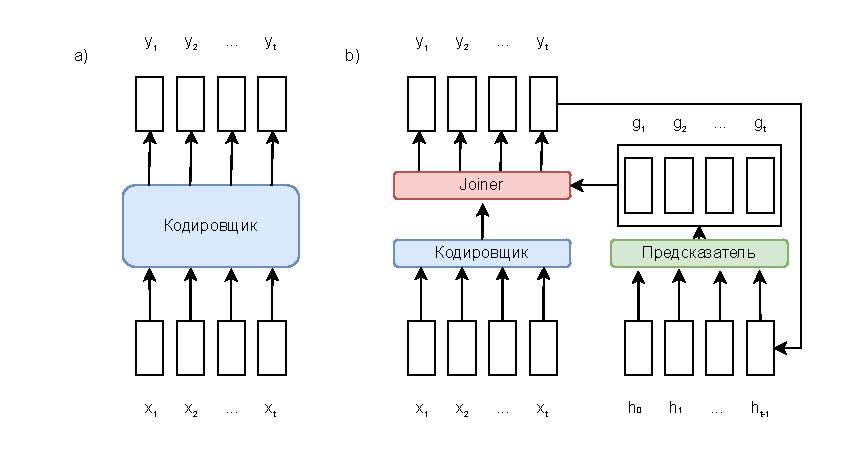
\includegraphics[width=160mm]{ctc_t.pdf}
  \caption{Архитектуры CTC (а) и Transducer (b).}
  \label{fig:ctc_t}
\end{figure}

В то время как CTC требует временного выравнивания, а RNN-T использует сложную систему совместного кодирования, LAS предлагает решение, основанное на механизме внимания.
Эта архитектура полностью отказывается от принудительного выравнивания аудио и текста, вместо этого динамически определяя соответствия между звуковыми фрагментами и символами выходного текста.
Кодировщик (listener) переводит аудио в скрытые состояния, внимание (attender) определяет релевантные участки звука для каждого символа, а декодер (speller) генерирует текст, учитывая взвешенные вниманием признаки и историю предсказаний.
Главное преимущество LAS перед CTC и RNN-T заключается в его способности напрямую моделировать сложные соответствия между звуком и текстом без необходимости явного временного выравнивания.
Механизм внимания позволяет системе гибко «перескакивать» между различными участками аудиосигнала, что особенно полезно при обработке речи с разной скоростью произношения или значительными паузами.

\subsection{Kaldi}
Одним из первых массовых решений, который занимал огромное место в области распознавания речи в 2010-х является Kaldi.
В дополнение к вышеописанной предобработке аудио сигнала модель применяет дискретное косинусное преобразование для получения Mel-Frequency Cepstral Coefficients (MFCC).
Далее каждая фонема моделируется как Марковская цепь (HMM) состояний.
Следом фреймы выравниваются с состояниями и подаются в глубокую нейронную сеть.
И далее с помощью BeamSearch происходит декодирование аудио через генерация текстовой последовательности.

\subsection{Рекуррентные ASR модели}
В 2014 выходит статья про архитектуру DeepSpeech от Baidu. 
Это модель, построенная на основе Recurrent Neural Network (RNN).
Их особенностью является возможность передачи скрытого состояния (hidden state) между ячейками одного слоя.
Это состояние представляет из себя своеобразный контекст подобно тому, как человек читает текст и связывает нынешнее слово с предыдущим.
Данные модели также можно «развернуть» и пустить в обратную сторону для закрепления полученных слов.
Происходит это за счёт создание дополнительного слоя такого же размера, но имеющим противоположное направление.
В Baidu как раз использовали двунаправленные (bidirectional) RNN.
Во второй версии DeepSpeech авторы сравнили два других подхода, основанных на вариантах RNN - Long-Short Term Memort (LSTM) и Gated Recurrent Unit (GRU).
Общим у этих подхов является механизм памяти, которые передаётся между ячейками.
С помощью забывания модели могут избавляться от информации, которую они считают не нужной или неактуальной.
Но эти механизмы в LSTM и GRU работают по разному.

LSTM приципиально отличает от RNN то, что она передаёт сразу два контекста: общий от предыдущих слов (long), который представляет собой информацию обо всей последовательности, и от последнего слова (short).
Благодаря этому LSTM-модели могут лучше чем RNN усваивать контекст и точнее решать задачи с длинными последовательностями.
Однако вместе тем это ведёт к повышенным затратам вычислительных ресурсов, поскольку механизм забывания устроен внутри достаточно сложно.
Основу механизма составляют 3 специальных фильтра: ворота (gate) забывания, входа и выхода.
Ворота забывания анализируют текущий вход и предыдущее состояние сети, чтобы принять решение о сохранении или удалении информации.
Математически этот процесс выражается через сигмоидную функцию, преобразующую входные данные в вектор значений от 0 до 1.
Каждое число в этом векторе действует как коэффициент сохранения для соответствующего элемента в памяти ячейки.
Когда значение близко к нулю, информация стирается, когда к единице — сохраняется в неизменном виде.
Затем ворота входа берут состояние прошлой ячейки, отбирают из неё информацию и передают в долгосрочную память.
И наконец ворота вывода берут информацию из долгосрочной памяти и прошлого скрытого состояния и создают новое скрытое состояние.

Для решения этой проблемы дорогих вычислений из-за наличия целых трёх вариантов ворот была создана архитектура GRU.
У неё, как и у RNN, существует только один вид памяти.
Ключевой особенностью GRU является ворот обновления (update gate), который одновременно выполняет функции как запоминания новой информации, так и забывания старой.
Этот ворот вычисляет, какая часть предыдущего состояния должна быть сохранена, а какая - заменена новыми данными.
Математически это выражается через комбинацию текущего входа и предыдущего скрытого состояния, пропущенных через сигмоидную функцию активации.
Механизм забывания в GRU работает по принципу плавного перехода между состояниями. Вместо полного стирания информации, как это иногда происходит в LSTM, GRU осуществляет взвешенное интерполирование между старым и новым состоянием. Это позволяет сохранять более устойчивые долгосрочные зависимости, избегая резких изменений в памяти сети.
На практике это означает, что GRU демонстрирует более стабильное поведение при работе с длинными последовательностями.
Так при обработке текста GRU может более плавно адаптироваться к изменениям контекста, постепенно ослабляя влияние устаревающей информации вместо её резкого отбрасывания.
Это особенно полезно в задачах, где контекст меняется постепенно, а не дискретно.

Интересно, что несмотря на упрощённую архитектуру, по итогу при правильной инициализации bias у gate GRU показывает сравнимую с LSTM производительность, а классические RNN обходит.
Механизм работы у GRU можно выразить уравнением~\ref{eq:gru}:

\begin{equation}
  \begin{aligned}
    z_t &= \sigma(W_z x_t + U_z h_{t-1} + b_z) \\
    r_t &= \sigma(W_r x_t + U_r h_{t-1} + b_r) \\
    \tilde{h}_t &= f(W_h x_t + r_t \circ U_h h_{t-1} + b_h) \\
    h_t &= (1 - z_t) h_{t-1} + z_t \tilde{h}_t
  \end{aligned}
  \label{eq:gru}
\end{equation}

\subsection{Пост-трансформерные модели}

\begin{figure}[!t]
  \centering
  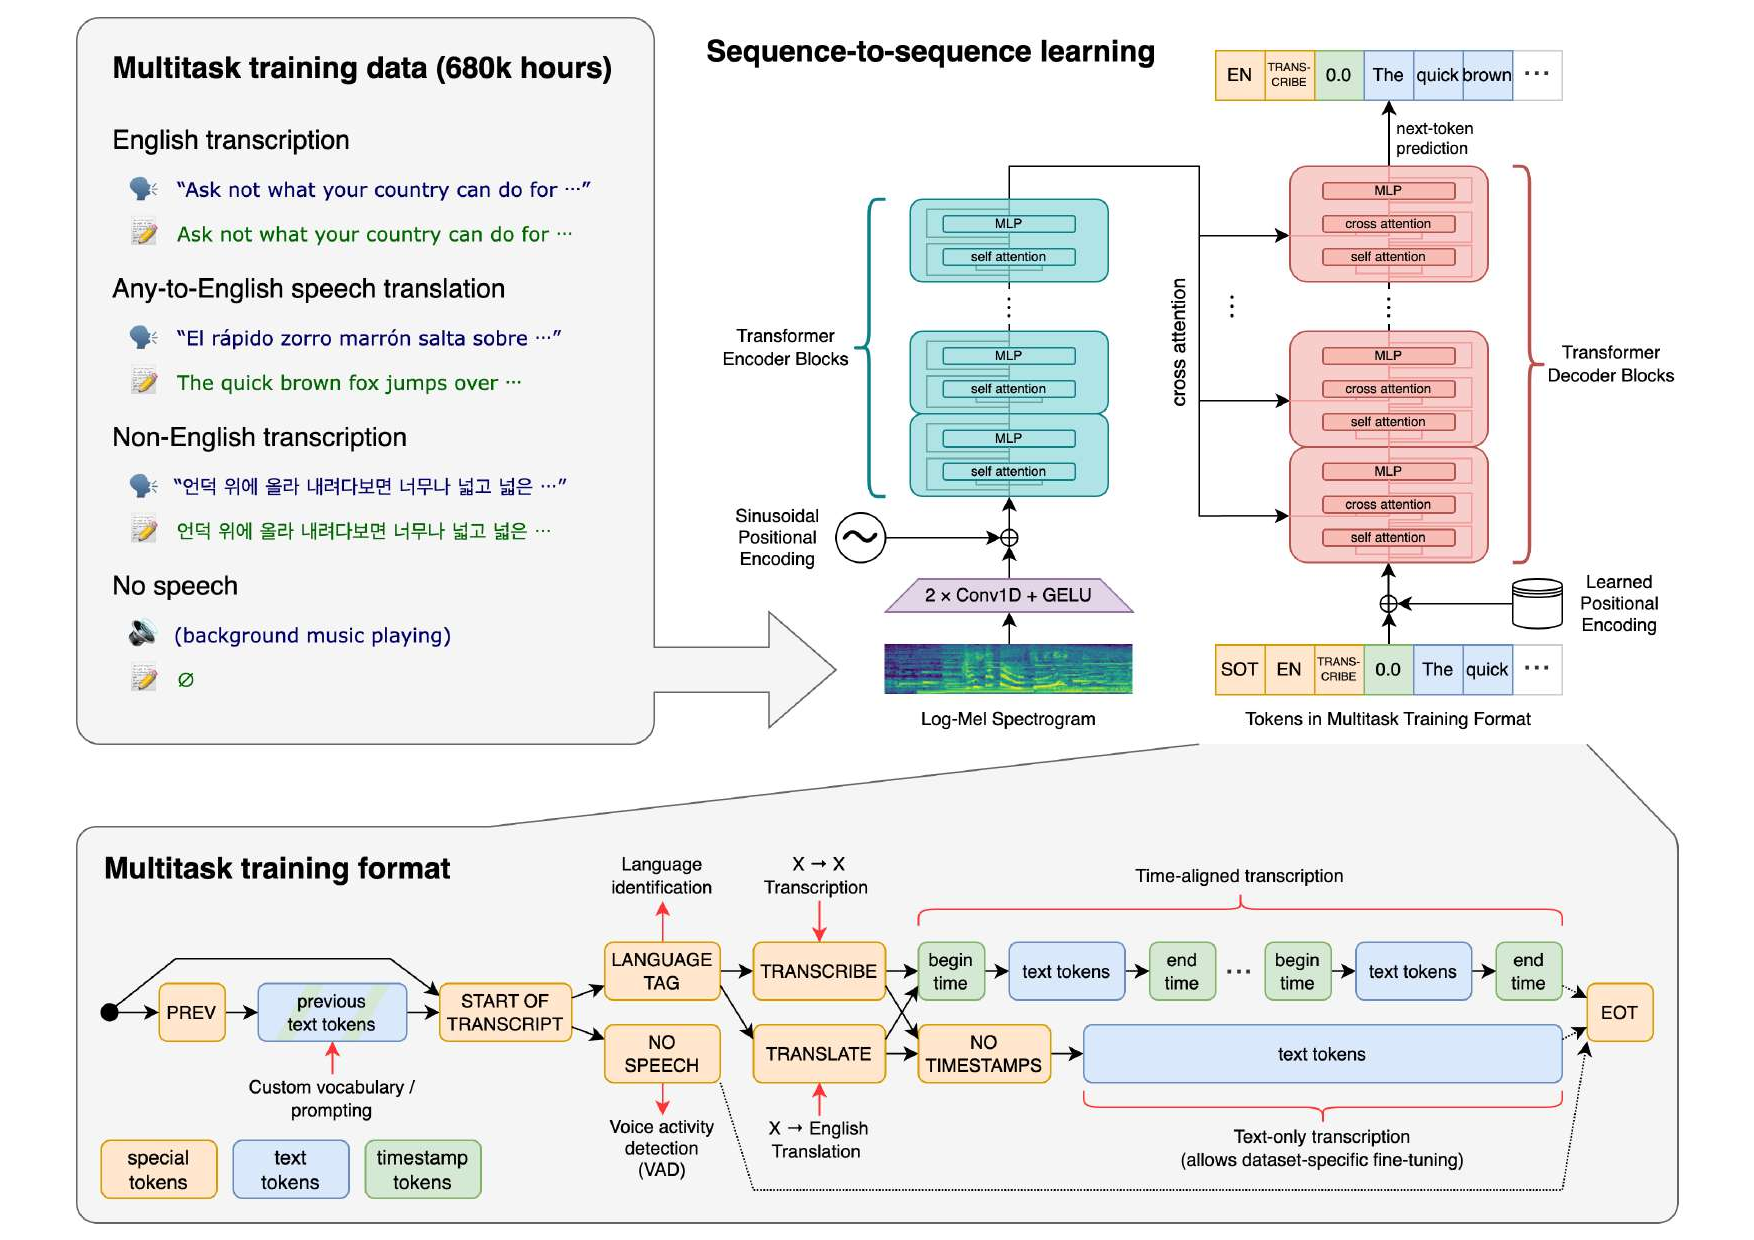
\includegraphics[width=140mm]{whisper.pdf}
  \caption{Архитектура модели Whisper.}
  \label{fig:whisper}
\end{figure}

Следующим большим словом в мире ASR систем стала модель Whisper от OpenAI, архитектура которой представлена на Рис.~\ref{fig:whisper}
Данная модель построена на основе архитектуры трансформер.
Эта архитектура была придумана Google в 2017 году в статье «Attention is all you need».
Суть архитектуры сводится к QKV attention механизму~\ref{eq:qkv}:

\begin{equation}
  \begin{aligned}
    Q &= W_Q \times X \\
    K &= W_K \times X \\
    V &= W_V \times X \\
    X &= Softmax(\frac{K^T \times Q}{\sqrt{d_h}}) \times V
  \end{aligned}
  \label{eq:qkv}
\end{equation}

Пусть у нас будет на вход матрица, состоящая из векторных представлений токенов $X$.
Мы умножаем её на матрицы весов $W_Q$, $W_K$ и $W_V$.
Так мы получаем наши матрицы Queries $Q$, Keys $K$ и Values $V$.
По своей сути их можно интерпретировать следующим образом:
\begin{itemize}
  \item Первая матрица отображает закодированное значение слов, к которым мы хотим добавить контекста последовательности.
  \item Вторая - значения, которые эти слова могут передать.
  \item Третья - дополнительную величину, на которую слова изменятся при добавление контекста.
\end{itemize} 

С помощью механизма внимания, трансформеры способны выделять локальные признаки в последовательности и создавать карты взаимозависимостей между отдельными токенами.
Если говорить про текстоый домен, то они выделяют зависимости между словами или их составными частями.

Модель Whisper разделёна на два блока: аудио энкодер и текстовый декодер.
Аудио энкодер свёрточной нейронной сетью (CNN) проходит по спектрограмме для выполнения предварительной обработкн и уменьшения размерности данных, подготавливая их для основного блока трансформера.
Свёрточные сети, придуманные в 1990 и использовавшиеся изначально с задачах компьютерного зрения Яном Лекуном в LeNet, проходятся окном свёртки по тензорам, выделяя какие-то общие визуальные паттерны.
Далее идут несколько слоёв трансформеров.
Ключевой особенностью этого энкодера является использование двунаправленных механизмов внимания, которые позволяют анализировать весь аудиоконтекст одновременно, в отличие от последовательных подходов RNN или ограниченных методов CTC.
Такая архитектура сохраняет исходное временное разрешение, избегая операций пулинга, что обеспечивает более точное сопоставление акустических признаков с текстовыми элементами.
Текстовый декодер же по своей работе  похож на методы рескоринга, о которых будем далее.
Можно сказать, что он представляет собой языковую модель (LM), которая авторегрессионно предсказывает следующий текстовый токен.
Она использует механизм внимания к энкодеру, что позволяет динамически определять наиболее релевантные участки аудиосигнала для генерации.
Мы делаем бесконечный цикл, передаём скрытое состояние декодера и предыдущие предсказанные слова, и генерируем новые до тех пор, пока не получим токен конца текста.
Языковая модель внутри Whisper обучена на огромном массиве многоязычных данных, что позволяет ей не только точно транскрибировать речь, но и учитывать контекст, исправлять омофоны и адаптироваться к разным акцентам.
Если в аудио встречается нечётко произнесённое слово, модель может восстановить его, опираясь на окружающий контекст.
Кроме того, Whisper способен работать с различными языками и даже переключаться между ними в рамках одного аудиопотока

Важным преимуществом Whisper является её универсальность - одна и та же архитектура успешно справляется с задачами распознавания речи, перевода и даже идентификации языка.
Это достигается за счет специальных токенов-инструкций, которые указывают модели требуемый тип обработки входных данных
Проблемой работы модели является то, что она не имеет моделей обученных исключительно для распознавания русского языка.
Существуют мультиязычные версии, однако они начинаются с модели Medium, в которой 700+ миллионов параметров.
Можно найти версии, которые были обучены членами ИИ-сообщества, однако зачастую такие модели обучаются на маленьком наборе данных из-за ограничений в вычислительных ресурсах у небольших команд.

\begin{figure}[!t]
  \centering
  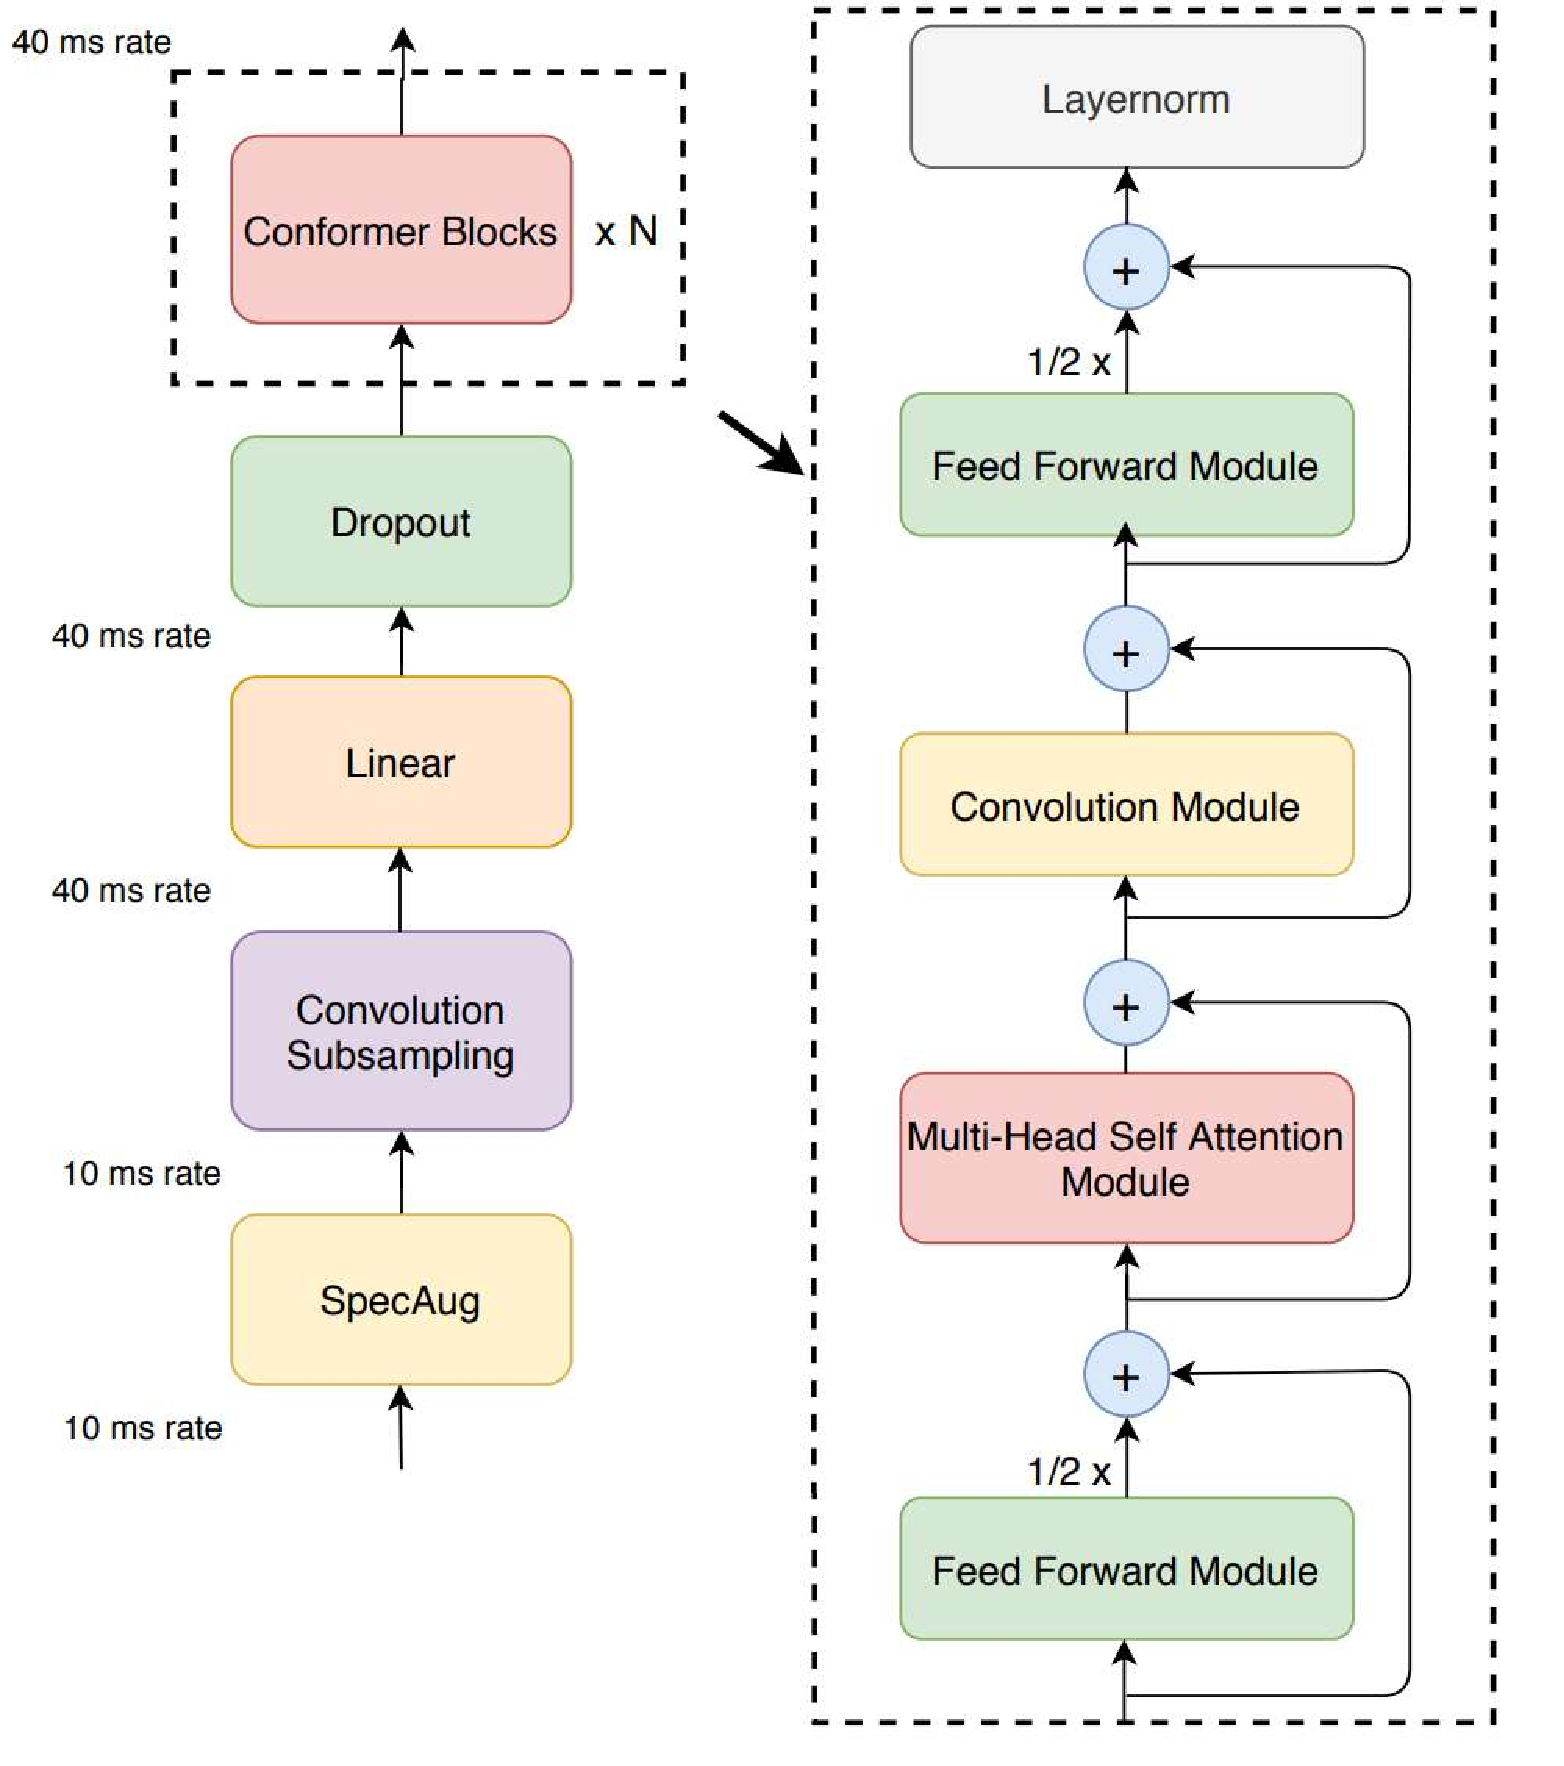
\includegraphics[width=100mm]{conformer.pdf}
  \caption{Архитектура модели Conformer.}
  \label{fig:conformer}
\end{figure}

Эту проблему решила Nvidia с выпуском серии FastConformer моделей. 
Они архитектурно построен на Conformer модели, архитектура которой показана на Рис.~\ref{fig:conformer}, где CNN используются в комбинации с трансформерами.
Как и в случае с Whisper спектрограмма изначально обрабатывается свёрточным слоем, однако отличием является то, что затем CNN будут дальше чередоваться с блоками трансформеров.
С помощью этой методики мы получаем карты активаций, на которых показано распределение визуальных признаков на нашем изначальном тензоре.
Грубо говоря, мы выделаем глобальные признаки из тензора с помощью свёрток.
А трансформеры, как мы говорил ранее, позволяют выделять локальные признаки из последовательности.
Благодаря объединению этих двух механизмов, мы получаем производительную архитектуру, которая хорошо улавливает все особенности аудио.
Проблему трансформеров, которые в силу своей архитектуры масштабируются квадратично, так как должны проверять зависимость токенов каждый от каждого, решили с помощью идей Longformer архитектуры.
Скользящее окно внимания и глобальный токен, в Nvidia ограничили «видимость» токенов в механизме внимания и уменьшили затраты вычислительных ресурсов.
Теперь каждый токен смотрит только на себя и на ближайших соседей.
Также модель обучалась с использованием Transducer архитектуры, где в качестве декодера выступает RNN-сеть, что позволяет достичь низкой задержки при обработке.


\section{Методы улучшения качества распознавания речи}
Когда заходит речь про адаптацию модели к какой-то задачи, первым на ум приходит доообучение этой самой модели на дополнительном большом наборе данных для обучения или же разработка новой архитектуры.
Мы не рассматриваем эти варианты по нескольким причинам.
Первый подход требует огромного количества вычислительных ресурсов для экспериметров с размерами, блоками модели.
Также он требует огромного количества данных.
Тут мы переходим к проблемам второго подхода.
Современные модели обучаются на огромном корпусе пар аудио-текст и добавив ещё данных мы разнообразим выборку новыми словами и в теории улучшим точность этого самого распознавания.
Но вместе с тем задача нахождения размеченного датасета пар аудио-транскрипция хорошего качества, ещё и на коротом модель не обучалась до этого - достаточно сложно.
Сюда же добавляется проблема того, что размеченные данные должны совпадать с теми, которые уже были использованы в обучение.
То есть наличие знаков препинания, совпадение регистра и правила написания чисел (цифрами или буквами).
Продолжим тем, что аудио сами по себе занимают много места в дисковом пространстве.
Если мы берём стандартное аудио, то есть частота дескритизации равна 16000 Гц.
Это значит, что одна секунда аудио кодируется 16000 числами.

Методы пост-коррекции начали появляться ещё до большого развития нейронных сетей.
Один из методов, который появился ещё 1990-е был ROVER.
Данная методика является своеобразным выравниванием (alighnment) гипотез.
При спользование этого метода, мы берём n-гипотез. 
Затем ROVER выравнивает все гипотезы относительно друг друга, чтобы согласовать их структуру.
Для этого используется подход, похожий на алгоритм динамического программирования, применяемый в задаче выравнивания последовательностей.
Каждая гипотеза представляет собой цепочку слов, и если их длины не совпадают, вставляются специальные пустые токены $\epsilon$, чтобы компенсировать расхождения в символах.
После попарного согласования всех гипотез формируется общая структура, где каждая позиция соответствует определённому месту в выровненной последовательности.
Если в какой-то гипотезе не хватает слова из-за разной длины, на его месте ставится пустой токен.
Мы проходим по токенам наших n-гипотез и проводим взвешенное голосование, в ходе которого определяется, какое слово войдёт в итоговый результат.
Учитывается частота появления каждого слова, а также вес гипотезы, из которой оно взято, если таковой имеется.
После голосования пустые токены отбрасываются, оставшиеся слова объединяются в итоговую строку.
Проблема данной методики заключается в том, что мы предполагаем, что наша ASR модель не имеет проблем с распознанием отдельным слов.
Если у нас в обучающих данных отсутствовало какое-то слово, то модель в теории может распознавать его хуже других.

Методом, который используется и в наши дни, является BeamSearch.
При жадом (greedy) декодирование это простейший подход, при котором на каждом шаге мы выбираем самый вероятный токен в качестве следующего элемента генерируемой последовательности.
Алгоритм жадный, потому что он не учитывает будущие шаги, а просто берёт лучшее на текущий момент.
Это быстро и эффективно по вычислительным ресурсам, но может приводить к неоптимальным результатам.
Может оказаться, что другая последовательность декодирования могла бы иметь большую вероятность, но ранний выбор закрыл путь к более удачным комбинациям.
BeamSearch в свою очередь пытается оптимизировать глобальную вероятность последовательности
При декодирование с его помощью мы одновременно строим и сохраняем несколько наиболее вероятных вариантов (beam) на каждом шаге.
Вместо того чтобы выбирать одно слово, алгоритм рассматривает несколько гипотез и развивает их параллельно.
На каждом шаге он расширяет эти гипотезы, оценивает их общую вероятность и оставляет только лучшие.
Всего одновременно существует $n$ последовательностей, где n - параметр $beam size$.
Мы делаем максимально вероятную последовательность, формула которой выглядит так~\ref{eq:probs}:
\begin{equation}
  P(y|x) = P(y|x_1,x_2,\dots x_n)
  \label{eq:probs}
\end{equation}

Таким образом на выходе мы получаем n последовательностей и их вероятностей.
В конце мы берём самую вероятную последовательность.
Это позволяет находить более качественные последовательности, но требует больше вычислений.
Проблема метода заключается в том, что он полагается на внутренние знания языка у модели транскрибации аудио.
Да и несмотря на более «разумную» генерацию мы не имеем гарантий, что такая стратегия покажет себя лучше жадного декодирования.

Другим методом улучшения качества распознавания, уже использующих языковые модели, является рескоринг (shallow fusion).
При этой методике, подобно Transducer, обучается внешняя языковая модель.
Суть в том, что LM может лучше оценивает естественность и грамотность предложений, чем основная модель ASR.
Берётся большой текстовый корпус, который кодируется токенизатором модели распознавания речи.
Затем обучается языковая модель на этом тексте.
Таким образом мы получаем LM, которая имеет внутреннее контекстное представление о вероятности следующего токена на основание предыдуших.
По своей сути тут решается уже задача уменьшения перплексии текстовой неопределённости.
Формулу рескоринга можно записать как~\ref{eq:rescore}:

\begin{equation}
  Score_{total} = \alpha Score_{ASR} + \beta Score_{LM},
  \label{eq:rescore}
\end{equation}
где $\alpha$ и $\beta$ коэффициенты веса.

LM вычисляет вероятность каждого предложения и корректирует итоговый рейтинг гипотез.
Часто используется взвешенная комбинация исходной вероятности от ASR и LM.
Но стоит помнить о необходимости подбора коэффициентов весов.
Такой подход помогает отфильтровать неестественные или грамматически неправильные варианты.

Один из классических способов реализовать рескоринг — использование n-граммной модели.
N-граммная LM предсказывает вероятность слова на основе предыдущих ($n-1$) слов.
В 3-gram модели вероятность каждого слова зависит от двух предыдущих.
Такие модели просты и эффективны в вычислительном плане, хотя и уступают нейросетевым LM в точности, поскольку не учитывают долгосрочные зависимости и опираются только на краткосрочные данные.
Для 3-gram модели формула предсказания токена будет выглядеть как в уравнение~\ref{eq:ngram}:
\begin{equation}
  P(x_i|x_{i-1},x_{i-2}) = \frac{Count(x_{i-2}, x_{i-1}, x_{i})}{Count(x_{i-2}, x_{i-1})}
  \label{eq:ngram}
\end{equation}

Нейросетевые LM анализируют всю последовательность целиком, что позволяет точнее предсказывать слова даже в сложных случаях (редкие термины, омофоны, сложный синтаксис).
Рекуррентные сети, такие как LSTM и GRU, обрабатывают текст последовательно, сохраняя информацию о предыдущих словах в скрытом состоянии.
Это позволяет им учитывать контекст при предсказании каждого следующего слова.
Однако их последовательная природа ограничивает параллелизацию и обработку очень длинных зависимостей между токенами.

Трансформерные архитектуры решают эту проблему с помощью механизма внимания, который анализирует все слова входной последовательности одновременно.
Self-attention позволяет модели напрямую устанавливать связи между любыми словами в тексте, независимо от расстояния между ними.
Это особенно полезно для распознавания сложных грамматических конструкций и редких терминов.

Преимуществом рескоринга является то, что он совместим и с другими методами улучшения качества распознавания речи, такими как ROVER или BeamSearch.
Если BeamSearch выдал гипотезу с редкой или странной комбинацией слов, n-граммная модель понизит её оценку, а более корректные варианты получат более высокий рейтинг.
Также найти качественный корпус текста в интернете сильно проще, чем размеченные аудио данные.
Вместе с тем его главным недостатком является завязанность на одной модели.
Мы не можем обучить языковую модель для рескоринга для разных ASR, поскольку LM строго завязана на токенизаторе.
То есть, если мы решим взять ту же модель, но при этом поменяем местами два токена, наша языковая модель будет бесполезна.

Deep Fusion представляет собой метод глубокой интеграции языковой модели LM в процесс распознавания речи, где взаимодействие между акустической и языковой моделями происходит на уровне скрытых представлений.
Этот подход существенно отличается от shallow fusion тем, что языковая модель влияет на процесс декодирования не только на финальном этапе, но и в процессе формирования промежуточных представлений.

\begin{figure}[!t]
  \centering
  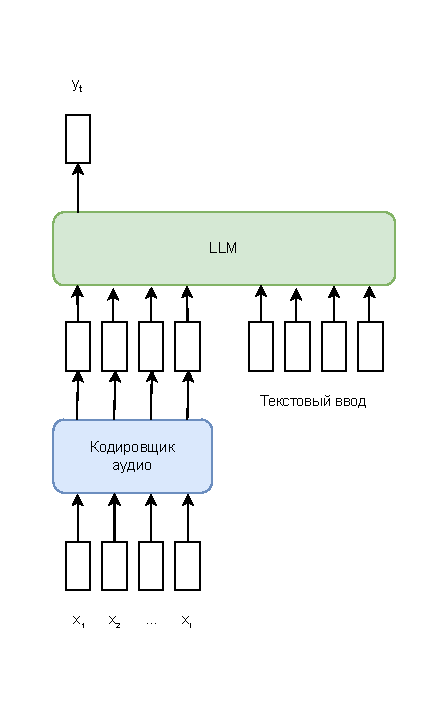
\includegraphics[width=80mm]{MLM.pdf}
  \caption{Мультимодальная модель с аудио кодировщиков.}
  \label{fig:mlm}
\end{figure}

Ещё одним варинатом объединения языковой модели с моделью распознавания речи стали Мультимодальные языковые модели, представленные на Рис.~\ref{fig:mlm}.
Multimodal LLM (MM-LLM) -- это класс моделей, способных одновременно обрабатывать и соотносить информацию из разных модальностей в рамках единой архитектуры.
В данном случае -- аудио и текст.
В контексте аудио такие модели не просто комбинируют готовые признаки из отдельных моделей, как в Deep Fusion, а изначально проектируются для совместного обучения на мультимодальных данных.
Объединение двух моделей -- кодировщика не лингистического домена, в нашем случае аудио, и лингвистической модели -- происходит за счёт коннектора, который обеспечивает взаимодействие между кодировщиками и языковой моделью.
Он переводит токены из домена энкодера в скрытое пространство языковой модели, где дальше уже языковая модель делает всё остальное.
LLM интерпретирует закодированную информацию как контекст и генерирует текстовый ответ или выполняет другую задачу, например, суммирование аудио или ответы на вопросы.
Важно, чтобы коннектор был обучен таким образом, чтобы сохранять важную информацию из аудио и преобразовывать её в форму, удобную для LLM.

Недостаток у этого подхода такой же, как у рескоринга - коннектор обучен переводить только из скрытого состояния одной модели распознавания речи в скрытое состояние одной языковой модели.
Плюсом для обучения кодировщика нам нужно делать прямые проходы через аудиокодировщик + языковую модель, а потом также делать обратный проход.
Это всё является очень затратными операциями, особенно если использовать LLM.
По той же причине мы отказываемся и от Deep Fusion.

Метод контекстного биазинга (context-biasing) --  позволяет улучшать распознавание редких и специализированных слов без необходимости модификации архитектуры модели или замедления процесса инференса.
Авторы статьи предлагают новый метод, основанный на использовании CTC-логарифмических вероятностей (log-probabilities) для сопоставления с компактным контекстным графом (Context Graph).
Этот граф строится на основе заранее заданного списка слов или фраз, требующих повышенного внимания при распознавании.
Как раз за счёт этого списка и идёт основной прирост в качестве.
Однако понятно, что метод сильно упирается в этот словарь.

Ключевая идея метода заключается в том, чтобы обнаруживать потенциальные кандидаты для биазинга и заменять ими соответствующие части жадного (greedy) декодирования.
Для моделей Transducer применяется гибридная архитектура Transducer-CTC, которая позволяет использовать CTC-WS без изменения исходной модели.
Контекстный граф основан на префиксном дереве (Trie), оптимизированном для хранения слов из списка биазинга.
Он учитывает особенности CTC-топологии, включая blank-переходы и self-loop для не-blank токенов, что делает поиск кандидатов более эффективным.

Алгоритм декодирования CTC-WS работает следующим образом: на каждом временном шаге он расширяет гипотезы, используя beam-search с параметрами $\beta_{thr}$ (blank) и $\gamma_{thr}$ (пропуск маловероятных токенов).
Для усиления влияния биазинга вводится контекстный вес (cbw), а при обработке перекрывающихся кандидатов выбираются наиболее вероятные варианты.

Минусами данного подхода можно выделить:
\begin{itemize}
  \item отсутствие учёта морфологии слов, так как разные формы слов требуют ручного добавления в граф
  \item сильная зависимость от CTC-выравнивания.
  \item проблемы с омофонами
  \item узконаправленность метода на улучшения в области, для которой отобраны фразы для графа
\end{itemize}

Теперь суммаризируем все вышеупомянутые ограничения методов.
Большинство из них так или иначе концентрируются на объединение языковой модели и модели распознавания речи.
Почти все, кроме ROVER, являются строго привязанными к определённой модели, то есть их знания не могут быть переданы для коррекции уже другой ASR.
Можно сравнить методы в сводной Таблице~\ref{tab:comp}

\begin{table}[]
\caption{Сравнение существующих методов улучшения качества распознавания речи.}
\label{tab:comp}
\begin{tabular}{|c|c|c|c|}
\hline
Метод                                                                       & \begin{tabular}[c]{@{}c@{}}Возможность\\ применять\\ к разным ASR\end{tabular} & \begin{tabular}[c]{@{}c@{}}Дополнительная\\ вычислительная\\ нагрузка\end{tabular} & \begin{tabular}[c]{@{}c@{}}Степень\\ прироста\\ качества\end{tabular} \\ \hline
BeamSearch                                                                  & +                                                                              & Низкая                                                                             & Низкая                                                                \\ \hline
ROVER                                                                       & +                                                                              & Низкая                                                                             & Низкая                                                                \\ \hline
\begin{tabular}[c]{@{}c@{}}Shallow Fusion\\ (N-Gram)\end{tabular}           & -                                                                              & Низкая                                                                             & Низкая                                                                \\ \hline
\begin{tabular}[c]{@{}c@{}}Shallow Fusion\\ (RNN, Transformer)\end{tabular} & -                                                                              & Средняя                                                                            & Средняя                                                               \\ \hline
Deep Fusion                                                                 & -                                                                              & Сильная                                                                            & Средняя                                                               \\ \hline
\begin{tabular}[c]{@{}c@{}}Мультимодальные\\ модели\end{tabular}            & -                                                                              & Сильная                                                                            & Сильная                                                               \\ \hline
Context-biasing                                                             & +                                                                              & Слабая                                                                             & \begin{tabular}[c]{@{}c@{}}Только в отдельных\\ темах\end{tabular}    \\ \hline
\end{tabular}
\end{table}

\section{Выводы}
В разделе была представлена общая информаци об области распознавания речи.
Была проведена комплексная оценка современных подходов, начиная от статистических мтеодов и заканчивая подходами на основе больших языковых моделей.
Выполнен детальный анализ эволюционного развития методов, выявлены ключевые ограничения существующих решений в области переносимости данных.
На основе сравнительного анализа установлены ограничения методов использования методов перехода из скрытого состояния ASR в скрытое состояние LM.